\documentclass{statsmsc}

\title{Comparing Aftershock Decay Functions for the 2019 Ridgecrest Earthquake 
Sequence}
\author{SACHIT RAMAKRISHNAN}
\CID{02032628}
\supervisor{ZAK VARTY}
\date{18 September 2026}

\logoimg{}

% THIS IS WHERE NEW COMMANDS CAN BE DEFINED

% commands below only used in the proof; otherwise can be deleted
\newcommand{\consta}{a}
\newcommand{\X}{X}
\newcommand{\EE}[1]{ \mathrm{E} [ #1 ] }
\newcommand{\inparenth}[1]{(( #1 ))}

\usepackage{xcolor}
\usepackage{float}
\usepackage{hyperref}
\hypersetup{
    colorlinks,
    linkcolor={blue!50!black},
    citecolor={blue!50!black},
    urlcolor={blue!50!black}
}

\defcitealias{scsn1926}{Caltech, 1926}
\defcitealias{scedc_changehistory}{SCEDC, 2026a}
\defcitealias{scedc_cataloguestatus}{SCEDC, 2026b}
\defcitealias{usgs_aftershocks}{USGS, 2025}

\defcitealias{scedc_format}{SCEDC, 2019}

\begin{document}

% Generates the Title Page
\maketitle

% Generates plagiarism declaration
\declarationname{SACHIT RAMAKRISHNAN}
\declarationdate{\today}
\declaration 

\begin{acknowledgements}
I would like to thank my supervisor, Zak Varty, for his guidance and feedback throughout this project. I am also grateful to the developers of \texttt{ETAS.inlabru} for making their software and source code available, which provided the computational framework extended in this project, and to the Southern California Earthquake Data Center for providing the earthquake catalogue used in this study. Most importantly, I would like to thank my family for their support throughout my studies.
\end{acknowledgements}

%=================================================================
% VERY IMPORTANT
% This command switches from Roman to Arabic numbering for main part of report. Do not modify.
\mainmatter
%=================================================================


\begin{abstract}
Following a large earthquake, the occurrence rate of nearby earthquakes rises sharply before gradually declining with time. This decay is conventionally described by the long-established Omori--Utsu law, although alternative mathematical forms have received empirical support and differ particularly in their behaviour over extended time horizons. This raises the question of how reliably they can be distinguished over the limited period covered by an earthquake catalogue. To address this, the present study compares three competing decay forms under finite-window conditions and assesses which is best supported by the 2019 Ridgecrest, California, earthquake sequence. This comparison is carried out within the epidemic-type aftershock sequence (ETAS) model, in which each earthquake increases the rate of subsequent events, using the \texttt{ETAS.inlabru} R package for approximate Bayesian inference. The existing inferential framework was extended beyond Omori--Utsu to include modified stretched exponential decay and the temporal response of a rate-and-state model. It was then evaluated in a known-truth synthetic experiment by fitting all three ETAS specifications to catalogues generated under each form before the extended framework was applied to Ridgecrest. The synthetic analysis showed that misspecified decay forms could reproduce the generating behaviour closely, yet marginal likelihood favoured the correctly specified form in almost all available comparisons. For Ridgecrest, marginal likelihood gave the strongest support to Omori--Utsu, with modified stretched exponential the closest competitor and rate-state considerably less supported. These findings show that similar fitted behaviour need not imply similar statistical support and that competing temporal decay forms can be distinguished over the finite-window conditions studied.
\end{abstract}

\section{Introduction} \label{sec:intro}

Earthquakes are among the most destructive natural hazards, causing substantial human and economic losses. Although the time, location, and magnitude of a future earthquake cannot be predicted \citep{geller1997earthquakes}, the elevated earthquake activity, or seismicity, following a large event can be modelled probabilistically \citep{Reasenberg1989}. The resulting earthquakes form a sequence in which the largest event is termed the mainshock and subsequent events are referred to as aftershocks. Since aftershocks may themselves trigger further events, the sequence can develop through successive generations of seismicity. The rate of triggered seismicity generally declines through time, with its temporal decay important for time-varying seismic hazard assessment \citep{hainzl2017testing}.

A standard framework for modelling such earthquake sequences is the epidemic-type aftershock sequence (ETAS) model, formalised by \citet{ogata1988statistical}. ETAS represents seismicity as a marked Hawkes process \citep{hawkes1971spectra}: a self-exciting point process in which each event increases the rate of future events and carries a mark -- its magnitude, a logarithmic measure of earthquake size. Its conditional intensity, the instantaneous event rate given the observed history, combines background seismicity, representing events not attributed to earlier activity, with triggering contributions from previous earthquakes. A magnitude-dependent productivity term controls the strength of each triggering contribution, while a temporal decay function determines how the contribution evolves through time. Since these effects accumulate across events, the Hawkes construction allows ETAS to represent secondary and higher-order aftershocks \citep{omi2015intermediate}.

Other approaches to modelling earthquake occurrence include statistical models such as the short-term earthquake probability model \citep{Gerstenberger2005}; physics-based models \citep{dieterich1994constitutive} combining friction theory with changes in mechanical stress on a fault, a zone of weakness in the Earth's crust along which rocks slip, producing earthquakes; and neural point processes that learn triggering relationships directly from data \citep{stockman2023forecasting, stockman2026earthquakenpp}. ETAS is adopted here because its temporal decay component can be varied while retaining a common self-exciting model structure, enabling direct comparison of alternative decay functions.

The conventional temporal decay function in ETAS is the empirical Omori--Utsu (OU) law \citep{omori1894aftershocks, utsu1961statistical, utsu1995centenary}, under which the aftershock rate follows a power law -- proportional to a negative power of the elapsed time since the triggering event. Two alternatives offer different physical interpretations: the modified stretched exponential (MSE) describes decay as a relaxation process, in which the elevated seismicity rate gradually returns towards its background level \citep{kisslinger1993stretched, gross1994tests}, while the rate-state (RS) function represents the temporal response implied by rate-and-state friction theory and transitions from approximately power-law to exponential decay \citep{dieterich1994constitutive, cocco2010sensitivity}. These forms differ most at long times, where OU permits more persistent triggering. In empirical comparisons within an ETAS framework, \citet{hainzl2017testing} found that the best-fitting form varied between sequences, with RS emerging as a strong alternative to OU.

These comparisons relied on maximum-likelihood estimation. For ETAS models, flat or multimodal likelihood surfaces can make numerical optimisation sensitive \citep{veen2008estimation}, while Hessian-based uncertainty estimates can be inaccurate when the observation window is limited \citep{wang2010standard}. Bayesian inference characterises parameter uncertainty through the posterior distribution, allowing uncertainty to be propagated to derived quantities such as the temporal decay function, but can be sensitive to prior specification. Recent Bayesian ETAS methods include a latent-variable MCMC scheme \citep{ross2021bayesian} and an approach by \citet{serafini2023approximation} based on integrated nested Laplace approximation \citep[INLA;][]{rue2009approximate}, a deterministic approximate Bayesian inference method. The INLA-based approach is implemented in the \texttt{ETAS.inlabru} R package \citep{naylor2023bayesian,naylor2023etas} and adopted here as a computationally efficient framework for fitting and comparing alternative temporal decay functions within a common temporal ETAS structure.

This framework is applied to the 2019 Ridgecrest, California, sequence using the Southern California Earthquake Data Center (SCEDC) catalogue \citeyearpar{scedc2013}. Its extensively recorded aftershock sequence \citep{hauksson2020ridgecrest} and multi-year post-mainshock record make Ridgecrest well suited to testing whether competing decay forms can be distinguished over a finite window. Both alternatives are relevant here: full rate-and-state formulations have performed well for Ridgecrest \citep{mancini2020predictive}, while relaxation-based decay forms have shown promise in California \citep{mignan2015modelling}.

This report makes three contributions. First, \texttt{ETAS.inlabru} is extended beyond Omori--Utsu by implementing the rate-state and modified stretched exponential decay functions. Second, known-truth synthetic catalogues generated under Ridgecrest-informed finite-window conditions assess how reliably the temporal forms are recovered and distinguished, including under model misspecification. Third, the extended framework is applied to the Ridgecrest sequence to compare fitted behaviour of the three decay functions, assess their relative support, and test the robustness of the resulting ranking.

The remainder of this report introduces the ETAS model and candidate decay functions in Section~\ref{sec:model}, followed by the Bayesian inference and model-comparison framework in Section~\ref{sec:inference}. Section~\ref{sec:study-design} describes the Ridgecrest catalogue and synthetic study design, Section~\ref{sec:study-results} presents the synthetic results, and Section~\ref{sec:ridgecrest} applies the framework to Ridgecrest. Section~\ref{sec:discussion} interprets the findings and their limitations.

\section{Modelling aftershock decay}\label{sec:model}

\subsection{The temporal ETAS model} \label{sec:etas} 

To compare temporal decay functions in a fixed region, earthquake occurrence is modelled using the temporal ETAS model \citep{ogata1988statistical}. Let $\left\{(t_i,m_i)\right\}$ denote a catalogue of events at times $t_i$ (in days) with magnitudes $m_i$, retained at or above a modelling magnitude threshold $M_0$, and let $\mathcal{H}_t = \left\{(t_j,m_j):t_j<t\right\}$ denote the event history before time $t$. Magnitudes are assumed independent and identically distributed according to the empirically motivated unbounded Gutenberg--Richter law \citep{gutenberg1944frequency}, 
\begin{equation} \label{eq:gr}
f_M(m) = \beta \, \exp \left\{-\beta(m-M_0)\right\}, \qquad \beta >0, \,m \geq M_0,
\end{equation}
where larger $\beta$ implies fewer large earthquakes. Event magnitudes are further assumed independent of their occurrence times and preceding history, an assumption that is standard in ETAS and has been found to hold reasonably well empirically \citep{schoenberg2004testing,stallone2019empirical}. Under this assumption, the magnitude and temporal likelihood components separate, allowing $\beta$ to be estimated from the catalogue and held fixed during temporal ETAS inference (Section~\ref{sec:eda}). 

Conditioning on the observed magnitudes, the temporal conditional intensity combines a constant background rate with triggering contributions from all preceding earthquakes:
\begin{equation*} 
\lambda(t \mid \mathcal{H}_t) = \mu+\sum_{(t_j,m_j) \in \mathcal{H}_t}K\exp\left\{\alpha(m_j-M_0)\right\} g(t-t_j), \qquad \mu, K >0, \, \alpha \geq 0.
\end{equation*}
The temporal decay function $g(\tau)$ is defined for elapsed time $\tau \geq 0$ and is non-negative, decreasing, integrable, and scaled so that $g(0)=1$. Under this scaling, the productivity term $K\exp\left\{\alpha(m_j-M_0)\right\}$ determines the initial rate of events triggered by event $j$, increasing exponentially with magnitude in accordance with empirical aftershock productivity relationships \citep{utsu1971aftershocks}. Here, $K$ sets this rate for an event of magnitude $M_0$, $\alpha$ controls its increase with magnitude, and $g(t-t_j)$ governs its decay. 

To relate this triggering rate to expected offspring over time, define the interval mass
\begin{equation*}
G(v,w) = \int_v^w g(\tau) \, \mathrm{d}\tau, \quad0\leq v < w \leq \infty.
\end{equation*}
An event of magnitude $m_j$ is expected to directly trigger $KG(v,w)\exp\left\{\alpha(m_j-M_0)\right\}$ events over elapsed times $[v,w]$. Taking the full event lifetime and averaging over the magnitude distribution gives the expected number of direct offspring per event, 
\begin{equation} \label{eq:branching}
\bar{n} = K  G(0,\infty) \mathbb{E}\left[\exp \left\{\alpha \left(M-M_0 \right) \right\} \right],
\end{equation}
also known as the branching ratio. Under Equation~\eqref{eq:gr}, the magnitude expectation is finite only for $\alpha < \beta$, giving $\bar{n} = K  G(0,\infty) \beta/(\beta-\alpha)$. The branching ratio determines the process's regime: the process is subcritical when $\bar{n} < 1$, so each event produces fewer than one direct offspring on average and triggered activity dies out rather than growing indefinitely \citep{helmstetter2002subcritical}. Despite this role in characterising triggering strength, the branching ratio does not enter the temporal likelihood, which conditions on observed magnitudes and remains well defined irrespective of the relationship between $\alpha$ and $\beta$.

More broadly, the simplifying assumptions of a constant background rate and temporal-only triggering provide a parsimonious framework for comparing temporal decay functions; their implications are discussed in Section~\ref{sec:discussion}.

\subsection{Temporal decay functions} \label{sec:decay}
Three contrasting temporal decay functions are selected from the broader comparison of \citet{hainzl2017testing}: Omori--Utsu as the conventional ETAS benchmark, with modified stretched exponential and rate-state as lighter-tailed alternatives. Their mathematical forms and tail behaviour are described below, with $g_k$ and $G_k$, respectively, denoting the decay function and interval mass for $k \in \{\mathrm{OU}, \mathrm{MSE}, \mathrm{RS}\}$; closed-form interval masses are given in Appendix~\ref{app:integrals}.

\subsubsection{Omori--Utsu decay} \label{sec:ou}

The inverse-time law of \citet{omori1894aftershocks} was generalised by \citet{utsu1961statistical} to allow a variable decay exponent, giving the Omori--Utsu law commonly used in ETAS \citep{ogata1988statistical}. Using the form implemented in \texttt{ETAS.inlabru} \citep{naylor2023bayesian}, 
\begin{equation*} 
g_{\mathrm{OU}}(t)  = \left(1+\frac{t}{c}\right)^{-p}, \qquad c>0, \;p>1.
\end{equation*}
The parameters $c$ and $p$ jointly control early-time decay, while $p$ determines the long-time power-law exponent. The restriction $p>1$ ensures integrability.  

\subsubsection{Modified stretched exponential decay} \label{sec:msexp}

\citet{kisslinger1993stretched} represented aftershock decay as a relaxation process in which a disturbed system gradually returns towards an equilibrium, producing stretched-exponential decay. \citet{gross1994tests} subsequently introduced the time offset $d$, analogous to the OU parameter $c$, producing the modified form used here.  

Under the convention $g_{\mathrm{MSE}}(0) = 1$, 
\begin{equation*} 
g_{\mathrm{MSE}}(t) = \left(1+\frac{t}{d} \right)^{\gamma-1} \exp \left\{ -\rho \left[(d +t)^{\gamma} - d^{\gamma}\right]\right\}, \qquad d >0, \: \rho >0, \: \,0< \gamma<1.
\end{equation*}
The parameters jointly determine the decay shape: larger $\rho$ produces faster decay, $\gamma$ controls how strongly the decay departs from a pure exponential, and $d$ primarily influences the early-time behaviour. As $\gamma \to 1$, the decay function approaches the pure exponential $\exp(-\rho t)$, while as $\gamma \to 0$, it approaches an OU form with $p = 1$. However, for any fixed $0 < \gamma <1$, it decays asymptotically faster than any power law but slower than any pure exponential.
 
\subsubsection{Rate-state decay} \label{sec:rs}

\citet{dieterich1994constitutive} derived the rate-and-state model from friction theory to describe how earthquake occurrence rates respond to changes in tectonic stress and relax towards their background level.  Following \citet{hainzl2017testing}, only its temporal response is retained here and rescaled so that $g_{\mathrm{RS}}(0) = 1$: 
\begin{equation*}
g_{\mathrm{RS}}(t) = \frac{(1 - B)\, \exp(-t / t_a)}{1 - B\exp(-t / t_a)}, \qquad 0 < B < 1, \; t_a > 0.
\end{equation*}
Here, $B$ is  related to the underlying stress perturbation and $t_a$ sets the relaxation time scale;  both are treated as decay-shape parameters rather than inferred from event-specific stress. At times short relative to $t_a$, the response is approximately OU with $p=1$, while at long times it approaches exponential decay \citep{cocco2010sensitivity}.

\subsection{Comparison of temporal decay functions} \label{sec:function-comparison}

\begin{figure} [H]
    \centering
    
\includegraphics[width=\linewidth]{images/decay-comparison.pdf}
    \caption{Comparison of (a) normalised decay densities and (b) survival functions using the parameter values based on \citet[Fig.~1]{hainzl2017testing}: $c = d = 0.01$ days, $p = 1.1$, $\rho = 1$, $\gamma = 0.2$, $B = 0.9999$, and $t_a = 100$ days.}
    \label{fig:decay-comparison}
\end{figure}

Figure~\ref{fig:decay-comparison} compares the temporal behaviour of the decay functions from two complementary perspectives: the normalised decay densities $f_k(t)=g_k(t)/G_k(0,\infty)$ and survival functions $S_k(t) = G_k(t,\infty)/G_k(0,\infty)$, where $S_k(t)$ gives the proportion of expected triggered events occurring after time $t$.

For the parameter values shown in Figure~\ref{fig:decay-comparison}, the functions are similar at short times but increasingly diverge at longer times, although the precise differences are parameter-dependent. More generally, their asymptotic behaviour remains structurally distinct: OU has a persistent power-law tail, MSE decays faster than any power law but slower than any pure exponential, and RS approaches exponential decay. How reliably they can be distinguished over a finite observation window is less clear; assessing this is a central aim of the study.

\section{Inference} \label{sec:inference}

\subsection{ETAS likelihood} \label{sec:likelihood}
Under the magnitude-separability assumption introduced in Section~\ref{sec:etas}, the temporal likelihood conditions on observed magnitudes, with the Gutenberg--Richter parameter $\beta$ estimated separately (Section~\ref{sec:eda}) and fixed. It is evaluated over a window $[t_\mathrm{start},t_\mathrm{end}]$, with $\mathcal{D}$ denoting events therein. By contrast, the history $\mathcal{H}_t$ may additionally contain events before $t_\mathrm{start}$, as their triggering contributions can extend into the window. 

For a temporal point process specified by a conditional intensity, the log-likelihood is the sum of log intensities at observed event times minus the integrated intensity over the fitting window \citep{ogata1988statistical}:
\begin{equation} \label{eq:loglik} 
\ell(\boldsymbol{\theta}; \mathcal{D}) =\sum_{(t_i, m_i) \in \mathcal{D}} \log  \lambda(t_i \mid \mathcal{H}_{t_i}) -  \int_{t_\mathrm{start}}^{t_\mathrm{end}} \lambda(t \mid \mathcal{H}_t)\,\mathrm{d}t,
\end{equation}
where $\log$ denotes the natural logarithm and $\boldsymbol{\theta}$ collects the background, productivity and decay parameters. Since the ETAS intensity is additive, the integrated intensity, or compensator, decomposes into background and event-specific triggering terms:
\begin{equation}\label{eq:compensator}
\Lambda = \underbrace{\mu (t_\mathrm{end} - t_\mathrm{start})}_{\Lambda_0} + \sum_{(t_j, m_j) \in \mathcal{H}_{t_\mathrm{end}}} \underbrace{K \exp\{\alpha (m_j - M_0)\} \, G\big(\max(t_\mathrm{start}, t_j) - t_j,\; t_\mathrm{end} - t_j\big)}_{\Lambda_j}.
\end{equation}
Combining the likelihood with the parameter priors defines the posterior, which is approximated using the INLA-based formulation of \citet{serafini2023approximation}, implemented in \texttt{ETAS.inlabru} by \citet{naylor2023bayesian}. INLA itself is introduced first (Section~\ref{sec:inla}), before the formulation that adapts it to the non-linear ETAS likelihood (Section~\ref{sec:inlabru}).

\subsection{INLA for latent Gaussian models} \label{sec:inla}

INLA \citep{rue2009approximate} performs approximate Bayesian inference for latent Gaussian models (LGMs). In an LGM, unobserved quantities form a Gaussian latent vector $\boldsymbol{z}$. The observations $\boldsymbol{y} = \{y_r\}_{r=1}^R$ are conditionally independent given $\boldsymbol{z}$, with each $y_r$ depending on $\boldsymbol{z}$ only through the corresponding component $\eta_r$ of the linear predictor vector $\boldsymbol{\eta}$:
\begin{equation*} 
 \boldsymbol{\eta} = A\boldsymbol{z}, \qquad \boldsymbol{z} \sim \mathcal{N}(\boldsymbol{0},Q^{-1}),
\end{equation*}
with $A$ a design matrix and $Q$ the precision matrix of $\boldsymbol{z}$ \citep{vanniekerk2023new}. In general, $Q$ and the likelihood may depend on hyperparameters over which INLA integrates numerically; the present formulation has none (Section~\ref{sec:reparam}), so this is omitted.

Inference targets the joint posterior $\pi(\boldsymbol{z} \mid \boldsymbol{y})\propto
\pi(\boldsymbol{y}\mid \boldsymbol{z})\,\pi(\boldsymbol{z})$, which is generally unavailable in closed form for non-Gaussian likelihoods. Laplace's method instead approximates the posterior around its mode $\widehat{\boldsymbol{z}}$ using a second-order expansion of its log-density \citep{tierney1986accurate}:
\begin{equation*}
\log \pi(\boldsymbol{z}\mid\boldsymbol{y})
\approx
\mathrm{constant}
-\frac{1}{2}
(\boldsymbol{z}-\widehat{\boldsymbol{z}})^\top
H
(\boldsymbol{z}-\widehat{\boldsymbol{z}}),
\end{equation*}
where $H$ is the negative Hessian of the log-posterior at the mode, giving the tractable joint Gaussian approximation
$\mathcal{N}(\widehat{\boldsymbol{z}},H^{-1})$. Because $\boldsymbol{\eta}$ is linear in $\boldsymbol{z}$ and each $y_r$ depends on $\boldsymbol{z}$ only through $\eta_r$, $H = Q+A^\top WA$, with diagonal $W$ containing the negative second derivatives of the log-likelihood contributions with respect to $\eta_r$ at the mode. When $Q$ and $A$ are sparse, INLA exploits this structure for efficient mode finding and construction of the Gaussian approximation \citep{rue2009approximate}. This approximation can, however, miss non-Gaussian features of individual marginals, which the original INLA formulation refines using further Laplace approximations \citep{rue2009approximate}, although these become costly when linear predictors greatly outnumber the latent components \citep{vanniekerk2023new}.

The present analyses used the R implementation of INLA \citep[R-INLA;][]{lindgren2015bayesian} in its compact formulation, which retains the joint Gaussian approximation and corrects its mean by a low-rank variational Bayes step \citep{vanniekerk2023new, vanniekerk2024lowrank}. Variational Bayes methods approximate a posterior by optimising over a tractable family of distributions \citep{blei2017variational}. When the posterior is asymmetric, its mean can differ from the mode, so here the correction shifts the Gaussian centre while retaining the Laplace covariance $H^{-1}$, with the shift estimated in a lower-dimensional space and propagated to the full latent vector. 

INLA is deterministic, avoiding Monte Carlo error and chain-convergence diagnostics, and can be markedly faster than MCMC for suitable LGMs \citep{rue2009approximate}. However, INLA relies on likelihood contributions depending on the latent Gaussian variables through linear predictors. ETAS intensities and integrated triggering contributions instead depend non-linearly on constrained model parameters, preventing direct application of standard INLA \citep{lindgren2024inlabru}. This motivates the \texttt{ETAS.inlabru} formulation described next.

\subsection{\texttt{ETAS.inlabru} formulation} \label{sec:inlabru}

\citet{serafini2023approximation} extend INLA to Hawkes processes through the \texttt{inlabru} R package \citep{bachl2019inlabru}, implemented for ETAS in the \texttt{ETAS.inlabru} package \citep{naylor2023bayesian}. Their approach represents constrained model parameters on a latent Gaussian scale and locally linearises the non-linear predictors entering the log-likelihood, so that the resulting LGM can be fitted using INLA. 

\subsubsection{Latent Gaussian parametrisation} \label{sec:reparam}
The first step maps the physical ETAS parameters $\boldsymbol{\theta}$ to a latent Gaussian scale $\boldsymbol{z}$. For each parameter,
\begin{equation*} 
z_q \sim \mathcal{N}(0,1), \qquad \theta_q = T_q(z_q) = F_q^{-1}\big(\Phi(z_q)\big),
\end{equation*}
where $\Phi$ and $F_q$ are the standard normal and target-prior cumulative distribution functions, respectively \citep{serafini2023approximation}. This permits constrained or non-Gaussian priors on the physical ETAS scale while retaining an unconstrained Gaussian latent representation. The components of $\boldsymbol{z}$ are independent, so $Q = I$ in the notation of Section~\ref{sec:inla}; the likelihood, however, remains non-linear in $\boldsymbol{z}$.

\subsubsection{Likelihood decomposition and temporal binning} \label{sec:decomp}
To prepare for linearisation, the log-likelihood is written, using Equations~\eqref{eq:loglik}--\eqref{eq:compensator}, in terms of the background compensator $\Lambda_0$, triggering compensators $\Lambda_j$, and event log intensities $\log\lambda_i$, where $\lambda_i = \lambda(t_i \mid \mathcal{H}_{t_i})$. A single linearisation of $\Lambda_j$ can be inaccurate over the full integration interval, so each $\Lambda_j$ is split into temporal bins that are narrowest after the parent event and widen with elapsed time \citep{serafini2023approximation}. The breakpoints are
\begin{equation*}
t_j,\; t_j + \Delta,\; t_j + \Delta(1 + \delta),\; t_j + \Delta(1 + \delta)^2,\; \ldots,\; t_\mathrm{end},
\end{equation*}
truncated to the fitting interval. Here, $\Delta$ and $\delta$ control the initial bin width and its growth, and $N_{\mathrm{max}}$ limits the number of geometric breakpoints, so parent $j$ has $N_j \leq N_{\mathrm{max}}+2$ bins and $\Lambda_j = \sum_{l=1}^{N_j} \Lambda_{j,l}$, where each bin mass is evaluated analytically. 

\subsubsection{Local linearisation} \label{sec:local-lin}

For each positive likelihood quantity $\psi_r(\boldsymbol{\theta})$, namely $\Lambda_0$, bin masses $\Lambda_{j,l}$ and event intensities $\lambda_i$, define the non-linear predictor $\eta_r(\boldsymbol{z}) =\log \psi_r \big(T(\boldsymbol{z})\big)$, where $T(\cdot)$ applies each $T_q(\cdot)$ component-wise. 
At the current linearisation point $\boldsymbol{z}^\ast$, \texttt{inlabru} uses the first-order approximation \citep{lindgren2024inlabru}
\begin{equation*}
\widetilde{\eta}_r(\boldsymbol{z};\boldsymbol{z}^\ast) = \eta_r(\boldsymbol{z}^\ast) + (\boldsymbol z-\boldsymbol z^\ast)^\top\nabla_{\boldsymbol{z}}\eta_r(\boldsymbol{z}^\ast).
\end{equation*}
Each approximation is affine in $\boldsymbol{z}$, giving the linear-predictor form of Section~\ref{sec:inla}, with the gradients $\nabla_{\boldsymbol{z}}\eta_r(\boldsymbol{z}^\ast)$ forming the rows of $A$ and the constant terms entering as a known offset. Relabelling the predictors by their likelihood quantities and substituting these approximations into the ETAS log-likelihood gives 
\begin{equation} \label{eq:approx-likelihood}
\widetilde{\ell}(\boldsymbol z;\boldsymbol z^\ast)
={}
-\exp\left\{
    \widetilde{\eta}_{\Lambda_0}
    (\boldsymbol z;\boldsymbol z^\ast)
\right\}-
\sum_{(t_j,m_j)\in\mathcal{H}_{t_\mathrm{end}}}\sum_{l=1}^{N_j}
\exp\left\{
    \widetilde{\eta}_{\Lambda_{j,l}}
    (\boldsymbol z;\boldsymbol z^\ast)
\right\} +
\sum_{(t_i,m_i)\in\mathcal D}
\widetilde{\eta}_{\lambda_i}
(\boldsymbol z;\boldsymbol z^\ast).
\end{equation}

\subsubsection{Iterative relinearisation} \label{sec:relin}
This linearisation is updated iteratively, starting from $\boldsymbol{z}^{\ast(0)}$, the latent-scale transformation of specified ETAS starting values. At iteration $s$, INLA fits the LGM linearised around ${\boldsymbol{z}}^{\ast (s)}$, yielding a candidate posterior mode $\widehat{\boldsymbol{z}}^{(s)}$. Because the first-order approximation is only locally accurate, \texttt{inlabru} uses a line search to choose how far to move towards the candidate mode \citep{lindgren2024inlabru}. This selects a step fraction $\xi$ to improve agreement between the non-linear predictors evaluated at the trial point and their linearised counterparts at the candidate mode, with discrepancies scaled by the linearised predictors' posterior standard deviations; $\xi = 1$ gives the full update. 

The chosen step gives the new linearisation point, where the predictors are relinearised and the resulting LGM is refitted using INLA. Convergence is declared when the line search no longer contracts the candidate update ($\xi \approx 1$) and the largest change in any latent parameter, relative to its current posterior standard deviation, satisfies
\begin{equation} \label{eq:convergence}
  \max_q \frac{|z_q^{\ast(s+1)}-z_q^{\ast(s)}|}{\mathrm{sd}^{(s)}(z_q \mid \mathcal{D})} < \epsilon.
\end{equation}
Otherwise, the procedure continues until convergence or the maximum number of iterations is reached \citep{lindgren2024inlabru}, with $\epsilon$ and the iteration limit specified as computational settings (Section~\ref{sec:numerical}). At the final linearisation point, the INLA fit provides the joint posterior approximation, from which latent marginals and joint samples are obtained and transformed to the physical ETAS scale. 

Thus, \texttt{inlabru} provides the outer iterative linearisation, while INLA performs approximate inference within each resulting LGM; outer convergence establishes stability of the linearisation point, not exactness of either approximation. 

\subsubsection{Extension to alternative decay functions} \label{sec:extension}
The existing \texttt{ETAS.inlabru} implementation is specific to the OU decay function \citep{naylor2023bayesian}. Here it is extended to the MSE and RS forms, retaining the binning, likelihood construction and iterative linearisation. For each new decay function, the extension requires its pointwise value $g_k(\tau)$ for the intensity, closed-form interval mass $G_k(v,w)$ for the compensator (Appendix~\ref{app:integrals}), and latent-scale transformations for its constrained parameters. Synthetic catalogue generation additionally requires the inverse cumulative mass of each decay function for sampling offspring times, as described in Section~\ref{sec:generation}.

Following \citet{serafini2023approximation}, the implemented decay functions are not normalised to unit integral, favouring a parametrisation more suitable for local linearisation. For the present comparison, each is scaled so that $g_k(0) = 1$ (Section~\ref{sec:etas}), giving $K\exp\{\alpha(m_j-M_0)\}$ a common interpretation as the initial triggering rate. Equal values of $K$ need not imply equal expected offspring numbers, since the integrated masses $G_k(0,\infty)$ differ.  

\subsection{Bayesian model comparison} \label{sec:model-comparison}

To assess relative support among the fitted temporal specifications, two criteria are used, both computed by INLA for the final linearised fit. The deviance information criterion \citep[DIC;][]{spiegelhalter2002bayesian} balances posterior model fit against effective model complexity:
\begin{equation*}
\mathrm{DIC} = \overline{\mathrm{Dev}}+p_D, \qquad
p_D = \overline{\mathrm{Dev}} - \mathrm{Dev}(\overline{\widetilde{\boldsymbol{\eta}}}).
\end{equation*}
Here, $\mathrm{Dev}(\widetilde{\boldsymbol{\eta}}) = -2\widetilde{\ell}$ is the deviance of the linearised log-likelihood (Equation~\eqref{eq:approx-likelihood}), up to a parameter-independent constant, $\overline{\mathrm{Dev}}$ is its posterior mean, and $\overline{\widetilde{\boldsymbol{\eta}}}$ is the posterior-mean vector of the linearised predictors \citep{rue2009approximate}. Smaller values are preferred.

For model $\mathcal{M}_k$ with parameters $\boldsymbol{\theta}_k$, the marginal likelihood is 
\begin{equation*}
\pi(\mathcal{D} \mid \mathcal{M}_k) = \int \pi(\mathcal{D} \mid \boldsymbol{\theta}_k, \mathcal{M}_k) \, \pi(\boldsymbol{\theta}_k \mid \mathcal{M}_k) \,\mathrm{d}\boldsymbol{\theta}_k,
\end{equation*}
which averages the likelihood over the model-specific prior $\pi(\boldsymbol{\theta}_k \mid \mathcal{M}_k)$. For the present formulation, INLA approximates the marginal likelihood of the final linearised model using the Gaussian approximation in Section~\ref{sec:inla}. For models $\mathcal{M}_1$ and~$\mathcal{M}_2$, the difference in their log marginal likelihoods (LML), $\Delta\mathrm{LML}_{12} = \log \pi(\mathcal D\mid\mathcal{M}_1)-\log \pi(\mathcal D\mid \mathcal{M}_2)$, is the log Bayes factor, with positive values favouring $\mathcal{M}_1$ \citep{kass1995bayes}. 

DIC and LML are evaluated on known-truth synthetic catalogues (Section~\ref{sec:synth-performance}) to determine which is retained as the primary criterion for Ridgecrest (Section~\ref{sec:ridgecrest}), with prior sensitivity examined separately (Section~\ref{sec:prior-sensitivity}).

\section{Data and experimental design} \label{sec:study-design}
Before fitting the competing decay forms to Ridgecrest, the extended computational framework was evaluated in a known-truth synthetic experiment under Ridgecrest-informed conditions to assess recovery of the generating form and discrimination between decay forms. To define these conditions, the observed catalogue was prepared by setting the spatio-temporal study window and magnitude threshold, then used to estimate the quantities informing the experiment. Synthetic catalogues were subsequently generated under each temporal decay function and fitted under all three forms, using pre-specified model-specific priors and numerical settings.

\subsection{Ridgecrest catalogue} \label{sec:eda}

\subsubsection{Sequence and catalogue} 

The 2019 Ridgecrest sequence began with an $M6.4$ foreshock\footnote{A foreshock is an earthquake that precedes the largest event in a sequence and is identified retrospectively once the mainshock occurs.} on 4 July, followed approximately 34 hours later by an $M7.1$ mainshock \citep{barnhart2019ridgecrest}. To capture both the sequence and pre-sequence seismicity that helps constrain the background rate \citep{naylor2023bayesian}, earthquake data from the Southern California Seismic Network \citepalias[SCSN;][]{scsn1926} were obtained through the Southern California Earthquake Data Center \citeyearpar[SCEDC;][]{scedc2013} for 1 January 2016 to 31 December 2025, without initial catalogue restrictions. This start date retains approximately 3.5 years of pre-sequence seismicity while avoiding documented catalogue-processing changes during 2015 \citepalias{scedc_changehistory}; the end date marks the last complete calendar year of processed data at the time of download in July 2026 \citepalias{scedc_cataloguestatus}.

During preprocessing, records with invalid coordinates, along with SCEDC-classified non-tectonic events, such as quarry blasts or sonic booms, were removed \citepalias{scedc_format}. Events flagged by the SCEDC as outside the SCSN local reporting area were also excluded; none lay within a conservative expected aftershock zone based on the Ridgecrest rupture extent \citep{barnhart2019ridgecrest} and typical spatial reach of aftershock sequences \citepalias{usgs_aftershocks}.

\subsubsection{Spatial window} 

The rectangular window of \citet{vanderelst2021bpositive}, $35.2 ^\circ$--$36.4 ^\circ$N and $118.2 ^\circ$--$117.0 ^\circ$W, was adopted to capture Ridgecrest seismicity while limiting unrelated activity (\hyperref[fig:ridgecrest-window]{Figure~\ref*{fig:ridgecrest-window}a}). Its northern boundary, for example, excludes the 2020 Lone Pine sequence, whose $M5.8$ mainshock \citet{Hauksson2021LonePine} concluded was not an aftershock of the Ridgecrest mainshock.

\begin{figure}[htbp]
  \centering
  \makebox[\linewidth][c]{
\includegraphics[width=\linewidth]{images/ridgecrest_window.pdf}}
  \caption{(a) Post-mainshock seismicity of all magnitudes in the Ridgecrest region; the dashed rectangle marks the adopted spatial window. (b) Post-mainshock seismicity rate for $M \geq 2.5$ events over successive three-month intervals; the dashed line marks the mean pre-sequence rate of 0.073 events/day.}
  \label{fig:ridgecrest-window}
\end{figure}

\subsubsection{Magnitude of completeness and analysis threshold} \label{sec:mag-complete}

The magnitude of completeness $M_c$ is the threshold at or above which earthquakes are assumed to be reliably detected \citep{woessner2005assessing}. Following large earthquakes, overlapping seismic signals can temporarily prevent smaller events from being detected, raising $M_c$ \citep{kagan2004short}. This short-term aftershock incompleteness (STAI) is evident around the Ridgecrest mainshock (\hyperref[fig:ridgecrest-completeness]{Figure~\ref*{fig:ridgecrest-completeness}a}) and can bias ETAS parameter estimates \citep{Hainzl2022}. Completeness was therefore assessed in daily windows around the Ridgecrest mainshock using candidate cut-offs spaced by $0.1$ magnitude units and three complementary diagnostics.

Maximum curvature \citep[MAXC;][]{wiemer2000minimum, woessner2005assessing} identifies the modal bin of the incremental frequency--magnitude distribution (\hyperref[fig:ridgecrest-completeness]{Figure~\ref*{fig:ridgecrest-completeness}b}). The other two diagnostics use the corresponding cumulative Gutenberg--Richter law, $N(m) \propto 10^{-bm}$, implied by the magnitude density in Equation~\eqref{eq:gr}, where $N(m)$ is the number of events with magnitude at least $m$ and $b = \beta /\log 10$. The goodness-of-fit test \citep[GFT;][]{wiemer2000minimum} selects the lowest candidate threshold $m^\ast$ for which the maximum-likelihood Gutenberg--Richter fit at that threshold has a summed absolute difference between observed and fitted cumulative counts of at most $10\%$ of the summed observed cumulative counts. The $b$-value stability method \citep[MBS;][]{cao2002temporal, woessner2005assessing} instead selects the lowest $m^\ast$ for which the estimated $b$-value differs from the mean of the $b$-value estimates over thresholds from $m^\ast$ to $m^\ast+0.5$ by no more than its standard error \citep{shibolt1982standard}. Both GFT and MBS use the bin-corrected Aki--Utsu maximum-likelihood estimator of $b$ \citep{aki1965maximum, utsu1965method, bender1983maximum}:
\begin{equation*}
\hat{b}(m^\ast)
=
\frac{\log_{10} e}
{\bar{m}(m^\ast)-\left(m^\ast-\frac{\Delta M_{\mathrm{bin}}}{2}\right)},
\end{equation*}
where $\bar{m}(m^\ast)$ is the mean magnitude of events with $m_i \geq m^\ast$ and $\Delta M_\mathrm{bin} = 0.01$ is the catalogue-specific magnitude discretisation.

On the day of the Ridgecrest mainshock, when incompleteness was most severe, MAXC estimated $M_c = 2.0$, whereas MBS and GFT gave higher estimates of $M_c = 3.3$ and $M_c = 3.2$, respectively. This divergence reflects the unusually flat frequency--magnitude distribution between $M1.5$ and $M2.5$ (\hyperref[fig:ridgecrest-completeness]{Figure~\ref*{fig:ridgecrest-completeness}b}).

A fixed threshold of $M_0 = 2.5$, lying between the MAXC and higher GFT/MBS estimates, was therefore adopted as a compromise between completeness and information retention; $M_0 = 3.3$ would reduce the catalogue from $3{,}339$ to $775$ events. The adopted threshold mitigates but does not eliminate STAI, which is considered when interpreting Ridgecrest results (Section~\ref{sec:mag-sensitivity}).

\begin{figure}[htbp]
    \centering
    
\includegraphics[width=\linewidth]
    {images/ridgecrest_completeness.pdf}
    \caption{Magnitude completeness at the onset of the Ridgecrest sequence (UTC). (a) Reported magnitudes, 2--14 July 2019. (b) Frequency--magnitude distribution on 6 July 2019, the day of the mainshock. Black dotted lines mark $M_0 = 2.5$. }
    \label{fig:ridgecrest-completeness}
\end{figure}

\subsubsection{Temporal window} 

Post-mainshock seismicity at or above $M_0$ declined but did not return to and remain at the mean pre-sequence rate of $0.073$ events/day (\hyperref[fig:ridgecrest-window]{Figure~\ref*{fig:ridgecrest-window}b}), so the full record was retained to maximise information on late-time decay, giving a window of $t_\mathrm{start} = -1282$ to $t_\mathrm{end} = 2371$ days relative to the mainshock at $t=0$, with no pre-window event history supplied. The Aki--Utsu estimate for this catalogue was $\hat{b}=0.865$, giving $\beta =1.992$. 

Together, $M_0$, $\beta$, the spatio-temporal window, the mainshock magnitude and the pre-sequence rate calibrate the synthetic catalogues.

\subsection{Synthetic benchmark design} \label{sec:design}

\subsubsection{Catalogue generation} \label{sec:generation}

Three data-generating specifications were defined, one for each temporal decay function. Each simulated events over the Ridgecrest window $t\in[-1282, 2371]$ days relative to an imposed $M7.1$ mainshock at $t=0$, with $M_0 = 2.5$ and $\beta = 1.992$. No pre-window events were supplied, so the pre-mainshock period contained background seismicity and its offspring only. 

Catalogues were generated using the branching simulator in \texttt{ETAS.inlabru} \citep{naylor2023bayesian}, extended here to MSE and RS forms. This exploits the Poisson-cluster representation of Hawkes processes \citep{hawkes1974cluster}: background events initiate clusters and triggered events form successive offspring generations, yielding a branching process equivalent to the ETAS conditional-intensity formulation. Under each specification, background events were generated from a homogeneous Poisson process of rate $\mu$: their count was Poisson-distributed with mean $\mu(t_\mathrm{end}-t_\mathrm{start})$ and times were sampled uniformly over the simulation window conditional on this count. Background magnitudes were sampled from a Gutenberg--Richter distribution with $\beta = 1.992$, truncated and renormalised over $M_0 \leq m \leq M_\mathrm{max}$, taking $M_\mathrm{max} = 7.1$ so that the imposed mainshock remained the sequence-defining largest event. These background events and the imposed mainshock then acted as parents in the branching process.

Each parent event $j$ generated a number of direct offspring from a Poisson distribution with mean 
\begin{equation*}
K\exp\{\alpha(m_j-M_0)\}G_k(0,t_\mathrm{end}-t_j). 
\end{equation*}
Conditional on this count, the offspring lags were obtained by inverse-transform sampling: writing $C_k(\tau) = G_k(0,\tau)$, a draw 
$\omega \sim \mathrm{Unif}(0,C_k(t_\mathrm{end} - t_j))$
was transformed to the lag $\tau = C_k^{-1}(\omega)$, with closed-form expressions for $C_k^{-1}$ given in Appendix~\ref{app:inverse}. This gave each offspring an occurrence time $t_j + \tau$, with a magnitude drawn from the truncated Gutenberg--Richter distribution. The resulting events then became new parents, with the procedure repeating recursively until no further events were generated. This procedure is common to the three specifications, which differ only through $G_k$ and $C_k^{-1}$.
\subsubsection{Generating parameters}
The parameters governing this branching process were specified to provide closely matched, Ridgecrest-informed sequences across the three generating forms. The background rate $\mu =0.073$ events/day was anchored to the empirical pre-sequence event rate rather than treated as an estimate of the ETAS background rate. The values $\alpha = 1.89$, $c = 0.03$ days, and $p = 1.17$ were adopted as Ridgecrest-informed anchors from \citet{kamranzad2025enhancing}, whereas $K$ was calibrated to an OU branching ratio (Equation~\eqref{eq:branching}) of $0.9$ under the truncated Gutenberg--Richter distribution and held common across forms, placing the simulated catalogues in a Ridgecrest-like event-count regime.

For the alternative forms, $t_a = 188$ days and $\gamma = 0.22$ were taken as characteristic RS and MSE values from \citet{hainzl2017testing}, while the MSE offset $d = 0.03$ days matched the OU short-time offset. The remaining parameters, $\rho$ and $B$, were chosen so that $G_{\mathrm{OU}}(0,t_\mathrm{end}) = G_{\mathrm{MSE}}(0,t_\mathrm{end}) = G_{\mathrm{RS}}(0,t_\mathrm{end}),$
giving $\rho = 1.959$ and $B$ within $10^{-4}$ of unity ($1-B = 8.5 \times10^{-5}$). With common $K$ and $\alpha$, this equalised the mainshock's expected direct offspring within the fitting window without collapsing the decay shapes (Figure~\ref{fig:synthetic-decay}). 

\begin{figure} [htbp]
    \centering
    
\includegraphics[width=\linewidth]{images/synthetic-decay-design.pdf}
    \caption{Generating temporal decay functions for the synthetic experiment. (a) $g_k(t)$; (b) cumulative triggering masses $G_k(0,t)$. The vertical dashed line marks the fitting window's end, $t=2371$ days, where masses were matched across forms.}
    \label{fig:synthetic-decay}
\end{figure}

\subsection{Fitting design}
With the generating design fixed, a common fitting setup was defined for the synthetic and baseline Ridgecrest analyses, comprising model-specific priors and initial values, and shared numerical settings.

\subsubsection{Prior and initial-value specification} \label{sec:priors}
Priors were defined on the physical ETAS parameters and chosen to be weakly informative, using previous studies to set plausible parameter scales without tightly constraining them (Table~\ref{tab:priors}). The priors for $\mu$, $K$, and the OU decay parameters followed \citet{naylor2023bayesian}, while the prior for $\alpha$ followed the scale-aware specification considered by \citet{serafini2023approximation}. MSE and RS decay-parameter priors were similarly informed by characteristic parameter values reported by \citet{hainzl2017testing}. 


\begin{table}[htbp]
\centering
\caption{Prior distributions and fixed initial values used for each candidate
model. Gamma($a$, $b$) has shape $a$ and rate $b$; lognormal and logit-normal distributions are parametrised by the mean and standard deviation
on the log and logit scales, respectively; $\iota=10^{-6}$ excludes boundary values.}
\label{tab:priors}
\begin{tabular}{llll}
\hline
Parameter & Prior & Initial value & Model \\
\hline
$\mu$     & Gamma$(0.5,0.5)$                    & $0.3$       & All \\
$K$       & Lognormal$(-1,0.5)$                 & $0.1$       & All \\
$\alpha$  & Gamma$(1,0.5)$ & $1$ & All \\
$c$       & Uniform$(\iota,1)$               & $0.2$       & Omori--Utsu \\
$p$       & Uniform$(1+\iota,2)$             & $1.1$       & Omori--Utsu \\
$d$       & Uniform$(\iota,1)$               & $0.2$       & Modified stretched exponential \\
$\rho$    & Lognormal$(\log 1.5,1)$             & $1$         & Modified stretched exponential \\
$\gamma$  & Uniform$(\iota,1-\iota)$      & $0.5$       & Modified stretched exponential \\
$B$       & Logit-normal$(7.5,1)$               & $100/100.2$ & Rate-state \\
$t_a$     & Lognormal$(\log 200,0.5)$           & $100$       & Rate-state \\
\hline
\end{tabular}
\end{table}

To assess whether the model-specific priors implied broadly comparable finite-window behaviour, $10{,}000$ joint draws from each were propagated to the finite-window mass $G_k(0,t_\mathrm{end})$ and normalised shape $h_k(t) = g_k(t)/G_k(0,t_\mathrm{end})$. The induced mass distributions had similar centres and strongly overlapping central 90\% intervals, while shape distributions remained broad and form-specific, with greater dispersion under MSE.

Initial values were likewise fixed before production fitting (Table~\ref{tab:priors}), using moderate interior values for the common and OU parameters following \citet{naylor2023bayesian}, with analogous interior values for the alternative temporal forms.

\subsubsection{Numerical settings} 
\label{sec:numerical}
Because the \texttt{ETAS.inlabru} approximation depends on the temporal binning of the triggering compensators (Section~\ref{sec:decomp}), numerical settings were calibrated on one pilot catalogue per form. Fixing the default binning geometry at $\Delta=0.1$ days and $\delta=1$, $N_{\mathrm{max}}$ was varied over $\{8,10,12,14,16\}$ to assess resolution. Posterior marginals and inferred decay functions stabilised by $N_\mathrm{max} = 14$, which was thus adopted. The convergence tolerance $\epsilon$ (Equation~\eqref{eq:convergence}) was then varied over $\{0.1, 0.05, 0.01 \}$; smaller values increased iteration counts without materially changing inference, so $\epsilon = 0.1$ was retained. The retained numerical settings are summarised in Table~\ref{tab:numerical-settings}.

\subsubsection{Production experiment}
With the fitting setup fixed, the generating design of Section~\ref{sec:design} was used to produce $100$ catalogues under each temporal form, giving $300$ synthetic catalogues. OU, MSE and RS were then fitted to each catalogue, giving $900$ candidate fits.

\begin{table}[htbp]
\centering
\caption{Numerical settings  for the synthetic and Ridgecrest analyses.}
\label{tab:numerical-settings}
\begin{tabular}{lc}
\hline
Setting & Retained value \\
\hline
Outer convergence tolerance $\epsilon$ & 0.1 \\
$N_{\mathrm{max}}$ & 14 \\
$\delta$ & 1 \\
$\Delta$ & 0.1 days \\
Maximum outer iterations & 100 \\
\hline
\end{tabular}
\end{table}
 
\section{Synthetic study results} \label{sec:study-results}

Since the underlying temporal decay form and parameters are unknown for Ridgecrest, the empirical analysis alone cannot establish whether the extended inferential framework can recover known temporal behaviour or reliably distinguish between competing forms. The known-truth synthetic study therefore provides a controlled assessment under Ridgecrest-informed finite-window conditions, considering numerical convergence, recovery under correct specification, behaviour under temporal-form misspecification, and model discrimination. These results inform the interpretation of the subsequent Ridgecrest analysis.
\subsection{Numerical convergence} \label{sec:reliability}

\begin{figure} [htbp]
    \centering
    
\includegraphics[width=0.6\linewidth]{images/convergence_3x3.pdf}
    \caption{Convergence across generating and fitted temporal forms. Values show the number of converged fits out of 100 for each combination. }
    \label{fig:convergence-heatmap}
\end{figure}

$781$ of $900$ production fits converged within $100$ outer \texttt{inlabru} iterations (Figure~\ref{fig:convergence-heatmap}). All $300$ correctly specified fits and most misspecified fits converged; RS fitted to MSE-generated catalogues was the clearest failure, with none of the $100$ fits converging.

Targeted post-hoc diagnostics indicated that this convergence instability was associated with RS fits entering a short-$t_a$ region when approximating MSE-generated decay. Increasing the variance of this parameter's lognormal prior produced little improvement, whereas recentring it towards shorter $t_a$ restored convergence in all $5$ test catalogues. The prospectively specified production prior was nonetheless retained because its location was informed by literature-supported RS timescales \citep{hainzl2017testing}. Subsequent model comparisons were therefore restricted to converged fits.

\subsection{Recovery under correct specification} \label{sec:recovery}
Recovery was gauged using the $300$ correctly specified fits, comprising $100$ catalogues under each temporal form. Parameters were considered first, followed by the temporal decay function jointly implied by them.

\subsubsection{Parameter recovery}

Parameter recovery was evaluated from three complementary perspectives: point-estimation accuracy, repeated-catalogue interval calibration, and posterior precision. Posterior medians were used as catalogue-level point estimates, with relative bias and root mean square error (RMSE) across catalogues calculated as a proportion of the generating value. Calibration was assessed by empirical coverage of $95\%$ credible intervals and precision by their median relative width. These summaries are reported in Table~\ref{tab:simulation-recovery}, with full posterior marginal distributions across catalogues provided in Appendix~\ref{app:posterior-recovery}.
\begin{table}[htbp]
\centering
\caption{Parameter recovery under correct specification across 100
synthetic catalogues per temporal decay form. Bias, RMSE and median 95\% credible-interval width are reported relative to the generating value; coverage is the proportion of 95\% credible intervals containing it; RS $B$
is reported as $1-B$.}
\label{tab:simulation-recovery}
\small
\begin{tabular}{llrrrr}
\hline
Form & Parameter & Rel. bias (\%) & Rel. RMSE (\%) &
Coverage (\%) & Rel. width (\%) \\
\hline
OU  & $K$      & -3.44 & 11.6 & 81 & 31.2 \\
    & $\alpha$ &  0.12 &  1.4 & 58 &  2.5 \\
    & $\mu$    &  5.45 & 12.6 & 70 & 24.6 \\
    & $c$      &  6.19 & 13.1 & 87 & 42.7 \\
    & $p$      &  0.56 &  1.3 & 76 &  3.2 \\
\hline
MSE & $K$      & -4.82 & 13.4 & 80 & 32.9 \\
    & $\alpha$ &  0.46 &  1.4 & 57 &  2.4 \\
    & $\mu$    &  0.19 &  7.0 & 90 & 23.9 \\
    & $d$      &  5.76 & 24.6 & 89 & 74.3 \\
    & $\gamma$ &  0.27 & 12.3 & 75 & 28.6 \\
    & $\rho$   &  1.48 & 14.3 & 83 & 35.3 \\
\hline
RS  & $K$      & -6.14 & 13.7 & 84 & 36.8 \\
    & $\alpha$ &  0.12 &  1.6 & 51 &  2.5 \\
    & $\mu$    &  3.09 &  10.5 & 78 & 24.3 \\
    & $1-B$    & 16.7  & 28.4 & 72 & 60.2 \\
    & $t_a$    & -5.24 & 13.9 & 62 & 21.5 \\
\hline
\end{tabular}
\end{table}

Point estimation errors were generally modest: absolute relative bias was below $10\%$ for all parameters with the exception of RS $1-B$ ($16.7\%$), while relative RMSE exceeded $15\%$ only for MSE $d$ ($24.6\%$) and RS $1-B$ ($28.4\%$). Interval calibration was weaker: with $100$ catalogues per generating form, binomial variation would place empirical coverage of a nominal $95\%$ interval in approximately the $90$--$99\%$ range, yet $15$ of $16$ parameters fell below this range. This was clearest for $\alpha$, whose relative RMSE was below $2\%$ under all temporal forms despite coverage of only $51$--$58\%$: posterior intervals for this parameter were systematically narrower than repeated-catalogue variability warranted. 

MSE $d$ showed a different pattern: its $24.6\%$ relative RMSE was accompanied by a $74.3\%$ median interval width and $89\%$ coverage, indicating that greater uncertainty was reflected in wider intervals. Among the form-specific decay parameters, calibration was weakest for RS; $t_a$ in particular showed a $5.2\%$ downwards bias and $62\%$ coverage. 

Overall, point estimation errors were limited for most parameters, but interval calibration and precision were uneven. To assess whether this affected the implied temporal behaviour, functional recovery was considered next.

\subsubsection{Functional recovery}

For each fit, $1{,}000$ joint posterior draws were used to evaluate $g_k(t)$ pointwise over the observation window, with each draw producing one posterior decay curve; their pointwise median defined the catalogue-level functional estimate. 

\begin{figure}
    \centering
    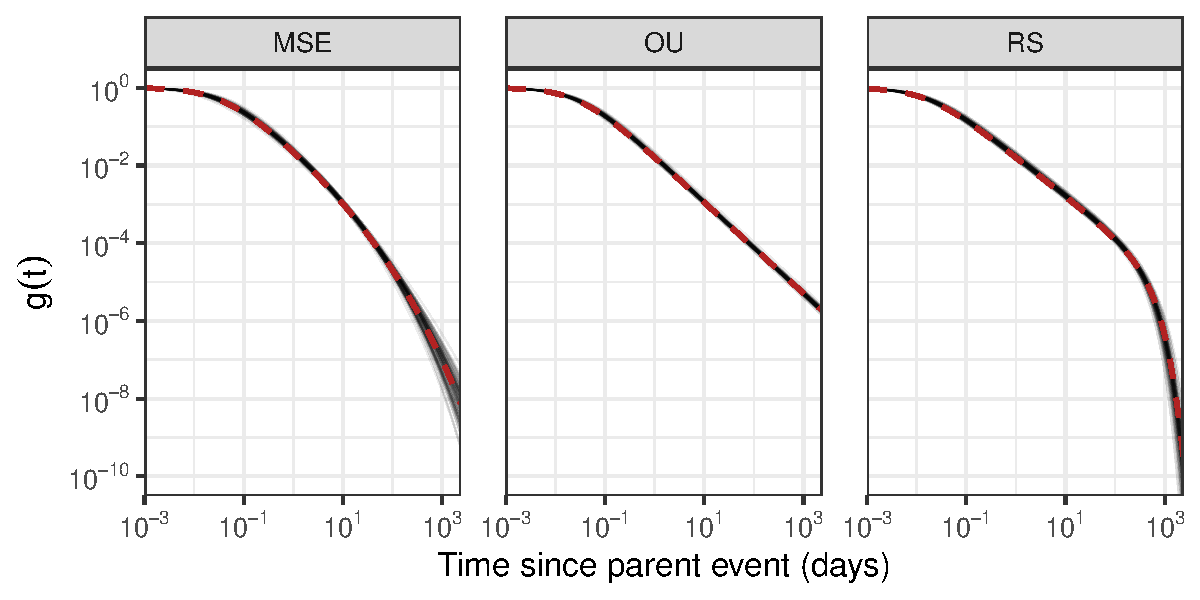
\includegraphics[width=0.8\linewidth]{images/functional_recovery.pdf}
    \caption{Functional recovery under correct specification. Grey lines show catalogue-level pointwise posterior-median estimates of $g_k(t)$; red dashed lines show corresponding generating functions over the fitted observation window.}
    \label{fig:functional-recovery}
\end{figure}

Figure~\ref{fig:functional-recovery} shows close recovery of the generating functions across all three forms, with greater late-time variation for MSE and, to a lesser extent, RS. Since logarithmic scaling can visually emphasise small absolute tail differences, recovery was additionally quantified using total-variation (TV) distance. Using the window-normalised shape $h_k(t)$ of Section~\ref{sec:priors}, the distance between fitted and generating shapes was defined as 
\begin{equation} \label{eq:tv}
    \mathrm{TV}(h_1,h_2) = \frac{1}{2}\int_0^{t_\mathrm{end}}|h_1(t)-h_2(t)| \,\mathrm{d}t.
\end{equation}
Under this definition, TV ranges from $0$ to $1$, with $0$ indicating identical  shapes and larger values indicating greater discrepancy. 

Median TV distances from the generating shape were $0.0165, 0.0123$, and $0.0123$ for MSE, OU, and RS, with $10$--$90$\% ranges of $0.0084$--$0.0258$, $0.0042$--$0.0259$, and $0.0046$--$0.0239$, respectively. Temporal shape was therefore recovered closely under all three forms, with similar TV-distance distributions. Across catalogues, pointwise coverage was calculated at each evaluation time as the proportion of $95\%$ credible intervals containing the generating value $g_k(t)$, then averaged over the evaluation grid. The resulting means were $83.9\%$, $91.9\%$, and $86.3\%$ for MSE, OU, and RS respectively, so functional calibration was closest to nominal for OU, with greater undercoverage for MSE and RS.

The stronger recovery of temporal decay functions relative to individual parameters was accompanied by strong posterior dependence among decay parameters. Median within-catalogue Spearman correlations were $0.74$ for OU $c$--$p$ and $-0.59$ for RS $(1-B)$--$t_a$, with the strongest MSE correlation reaching $-0.96$ for $\gamma$--$\rho$. These dependencies were consistent across catalogues (Appendix~\ref{app:posterior-correlation}) and suggest that decay parameters can vary together while implying similar functional shapes. 

Hence, despite uneven scalar recovery and calibration, the jointly implied temporal decay was recovered more consistently.

\subsection{Functional behaviour under temporal-form misspecification} \label{sec:misspecification}
Given the close functional recovery under correct specification, the next question is how closely misspecified forms can reproduce the generating behaviour. 

\begin{table} [t]
\centering
\caption{Functional overlap under temporal-form misspecification. Positive $\Delta \mathrm{TV}$ values indicate that the correctly specified form is closer to the generating shape.}
\label{tab:misspec-tv} 
\begin{tabular}{llrrrr} 
\hline
Truth & Alternative & $n$ & Median $\Delta \mathrm{TV}$ & 10--90\% & Alternative closer \\
\hline
MSE & OU  & 100 & 0.0544 & 0.0445--0.0644   & 0.0\% \\
OU  & MSE & 97  & 0.0101 & 0.0029--0.0179 & 5.15\% \\
OU  & RS  & 100 & 0.1143 & 0.1027--0.1223   & 0.0\% \\
RS  & MSE & 84  & 0.0379 & 0.0303--0.0438   & 0.0\% \\
RS  & OU  & 100 & 0.0996 & 0.0860--0.1158   & 0.0\% \\
\hline
\end{tabular}
\end{table}

To assess functional similarity under misspecification, the pointwise posterior-median temporal decay function from each misspecified fit was compared with the generating function using the window-normalised TV distance of Equation~\eqref{eq:tv}. For each catalogue, the difference from the corresponding correctly specified distance was defined as
\begin{equation*}
\Delta\mathrm{TV} = \mathrm{TV}(h_{\mathrm{true}}, \hat{h}_{\mathrm{alt}}) - \mathrm{TV}(h_{\mathrm{true}}, \hat{h}_{\mathrm{true}}).
\end{equation*} 
Values near zero indicate the alternative reproduces the generating shape almost as closely as the correct form, while negative values indicate it is closer. 

The degree of functional similarity varied markedly between model pairs (Table~\ref{tab:misspec-tv}). MSE provided the closest misspecified approximation to OU truth, with median $\Delta \mathrm{TV}=0.0101$ and posterior-median curve closer to the generating shape than the corresponding OU curve in $5.15\%$ of catalogues. The reverse comparison showed less overlap, while OU--RS comparisons showed much greater separation; RS fits to MSE truth are absent, as discussed in Section~\ref{sec:reliability}. 

The preceding comparisons reduced each functional posterior to its pointwise median curve, quantifying similarity of the central fitted shape but not variation in temporal shape across the posterior. TV distance from the generating function was thus also calculated for each of the $1{,}000$ joint posterior draws, with each normalised separately over the fitting window. The median-based pattern persisted across the posterior (Appendix~\ref{app:posterior-functional-tv}), with MSE fitted to OU truth the only misspecified combination whose posterior TV distances approached those of the correctly specified fit; this similarity may reflect the greater flexibility of MSE's three-parameter decay form. 

Functional similarity therefore does not by itself identify the generating form, providing a demanding test for formal model discrimination in the following section.

\subsection{Model discrimination under known truth} \label{sec:synth-performance}
DIC and marginal likelihood (Section~\ref{sec:model-comparison}) were evaluated under known truth, with discrimination assessed using selection frequency and pairwise criterion differences.

Three-way comparisons required all three fits to converge and were therefore available for $97$ OU- and $84$ RS-generated catalogues. Marginal likelihood selected the correctly specified temporal form for all $84$ RS cases and $96$ of $97$ OU cases, whereas DIC selected RS in every comparison and was thus consistently incorrect under OU truth. The pairwise results in Figure~\ref{fig:pairwise-model-comparison} reinforced this contrast: DIC systematically favoured the misspecified alternative under OU truth, despite favouring the correctly specified form in available MSE- and RS-generated comparisons. 

\begin{figure} [H]
    \centering
    
\includegraphics[width=\linewidth]{images/pairwise_model_comparison.pdf}
    \caption{Pairwise model-comparison differences for (a) DIC and (b) log marginal likelihood. Boxes show medians and interquartile ranges; positive values favour the correctly specified form.}
    \label{fig:pairwise-model-comparison}
\end{figure}
Unlike the three-way analysis, pairwise comparisons required only the two relevant fits to converge. Marginal likelihood favoured the correctly specified form in all but two available pairwise comparisons, although evidence strength varied between model pairs. Table~\ref{tab:lml-pairwise} shows that separation was weakest for OU truth against MSE, with median $\Delta\mathrm{LML}$ $= 3.34$ and a lower decile of $1.97$. The two incorrect selections also occurred in opposite directions between OU and MSE: once under OU truth ($\Delta\mathrm{LML}$ $=-1.37$) and once under MSE truth ($\Delta\mathrm{LML}$ $=-0.54$). Thus, the strongest functional similarity identified in Section~\ref{sec:misspecification} coincided with the weakest marginal-likelihood separation, yet the correctly specified form was still favoured in $96$ of $97$ OU-generated comparisons. This contrast may partly reflect marginal likelihood accounting for fit across the model's prior-weighted parameter space, rather than the closeness of the fitted temporal decay function alone.

\begin{table}[htbp]
\centering
\caption{Pairwise marginal-likelihood discrimination under known generating temporal form. Positive $\Delta\mathrm{LML}$ values favour the correctly specified form.}
\label{tab:lml-pairwise}
\begin{tabular}{llrrrr}
\hline
Truth & Alternative & $n$ & Truth favoured & Median $\Delta\mathrm{LML}$ & $10$--$90\%$ \\
\hline
OU  & MSE & 97  & 99\% & 3.34 & 1.97--4.23 \\
OU  & RS  & 100 & 100\% & 48.4 & 26.6--96.3 \\
MSE & OU  & 100 & 99\%  & 13.8 & 3.94--32.0 \\
RS  & OU  & 100 & 100\% & 46.6 & 23.6--79.6 \\
RS  & MSE & 84  & 100\% & 14.5 & 9.38--21.1 \\
\hline
\end{tabular}
\end{table}
These results motivated the use of marginal likelihood as the primary model-comparison criterion in the Ridgecrest analysis.

\section{Ridgecrest}\label{sec:ridgecrest}
The analysis now turns to the observed Ridgecrest catalogue, for which the underlying temporal decay form is unknown. Baseline posterior inference and posterior-implied temporal behaviour are examined first, followed by comparison of relative model support and assessment of the robustness of the resulting conclusions.
\subsection{Baseline analysis}

For the baseline analysis, $3{,}339$ events at or above $M_0 = 2.5$ were retained over the observation window, $t\in[-1282,2371]$ days relative to the $M7.1$ mainshock, defined in Section~\ref{sec:eda}. The three ETAS specifications, differing only in temporal decay form, were fitted to this catalogue using the same inferential framework, priors, and numerical settings as in the synthetic study. All three fits converged within $100$ outer \texttt{inlabru} iterations.
\subsubsection{Posterior parameter inference}
Marginal posterior summaries for the model parameters are shown in Table~\ref{tab:ridgecrest-posterior}.  The magnitude-scaling parameter $\alpha$ had similar posterior distributions across all three specifications, with greater between-model variation in the background rate $\mu$ and productivity parameter $K$, whose posterior medians were larger under RS than under OU or MSE. 

\begin{table}[htbp]
\centering
\caption{Posterior parameter summaries for Ridgecrest baseline fits. Posterior medians are reported with 95\% credible intervals (CrI).}
\label{tab:ridgecrest-posterior}
\small
\begin{tabular}{llcc}
\hline
Model & Parameter & Median & 95\% CrI \\
\hline
OU  & $\mu$        & 0.0553 & (0.0481, 0.0633) \\
OU  & $K$          & 1.32   & (1.12, 1.55) \\
OU  & $\alpha$     & 1.96   & (1.94, 1.98) \\
OU  & $c$          & 0.0211 & (0.0172, 0.0257) \\
OU  & $p$          & 1.22   & (1.20, 1.24) \\
\hline
MSE & $\mu$        & 0.0592 & (0.0518, 0.0675) \\
MSE & $K$          & 1.39   & (1.13, 1.73) \\
MSE & $\alpha$     & 1.97   & (1.95, 1.99) \\
MSE & $d$          & 0.0167 & (0.0115, 0.0240) \\
MSE & $\rho$       & 4.40   & (2.14, 9.03) \\
MSE & $\gamma$     & 0.0564 & (0.0251, 0.112) \\
\hline
RS  & $\mu$        & 0.0902 & (0.0809, 0.100) \\
RS  & $K$          & 2.27   & (1.81, 2.85) \\
RS  & $\alpha$     & 1.98   & (1.96, 2.00) \\
RS  & $1-B$        & $7.37\times10^{-5}$ & ($5.48\times10^{-5}$, $9.89\times10^{-5}$) \\
RS  & $t_a$        & 66.9   & (59.7, 74.8) \\
\hline
\end{tabular}
\end{table}

For the model-specific decay parameters, the RS fit is particularly notable: the posterior concentrated on a relatively short relaxation time, with median $t_a = 66.9$ days and $95\%$ credible interval $(59.7, 74.8)$ days, well below the centre of its literature-informed prior. This estimate should nevertheless be interpreted cautiously, since $t_a$ showed undercoverage in the synthetic study. More generally, the synthetic results motivate examining the Ridgecrest temporal behaviour through the joint posterior-implied decay functions rather than individual parameters.

\subsubsection{Temporal decay behaviour}
For each fit, $10{,}000$ joint posterior draws were propagated through the corresponding decay function and evaluated over the fitting window, yielding pointwise posterior medians and $95\%$ credible intervals calculated across draws. Both the unnormalised function $g_k(t)$  and the window-normalised function $h_k(t)$ were considered, providing complementary views of temporal behaviour: the former compares temporal decay on the common scale $g_k(0) =1$, while the latter isolates differences in the relative timing of triggering over the observation window.

\begin{figure}
    \centering
    
\includegraphics[width=1\linewidth]{images/ridgecrest-functional-posteriors.pdf}
    \caption{Posterior-implied temporal decay for the baseline Ridgecrest fits. Lines show posterior medians and shaded regions show $95\%$ pointwise credible intervals from $10{,}000$ posterior draws. (a) Unnormalised $g_k(t)$; (b) window-normalised $h_k(t)$.}
    \label{fig:ridgecrest-functional-posterior}
\end{figure}

Figure~\ref{fig:ridgecrest-functional-posterior} shows 
clear similarity between the fitted OU and MSE temporal decay functions. Their posterior-median $g_k(t)$ curves remain close across most of the fitted window, with similarly narrow posterior uncertainty, and minor discrepancies only emerging towards the analysis cut-off. On the other hand, the RS curve is lower over much of the early and intermediate range and exhibits a noticeably sharper decline at longer times. Since all temporal decay forms satisfy $g_k(0) = 1$, the lower RS curve reflects a smaller triggering contribution at these lags for a given $K$; because the posterior for $K$ differed between fits, this does not itself imply lower total triggering under RS.

After normalisation, OU and MSE remain close throughout the window, whereas RS shows a more distinct shape: it starts higher, falls below them within the first day, rises above them over intermediate lags, and declines below them after approximately $100$ days as its asymptotically exponential behaviour becomes dominant.

The close MSE--OU agreement echoes the finite-window similarity observed in the synthetic study, where MSE fits could approximate OU-generated temporal decay closely. As the synthetic results showed, such functional similarity need not translate into similar model support, which is assessed next using marginal likelihood.

\subsubsection{Model comparison}

Following its reliable known-truth discrimination in Section~\ref{sec:synth-performance}, marginal likelihood was used to compare relative support among the three candidate ETAS specifications (Table~\ref{tab:ridgecrest-model-comparison}). The OU--MSE difference was $\Delta\mathrm{LML} = 3.51$, corresponding to a Bayes factor of $33.6$ in favour of OU. Differences involving RS were much larger: $\Delta\mathrm{LML} = 96.61$ for OU and $93.10$ for MSE against RS. Within the candidate set, OU received the greatest relative support, followed by MSE, while RS received substantially less support than either alternative.
\begin{table}[htbp]
\centering
\caption{Marginal-likelihood comparison for the baseline Ridgecrest fits. $\mathrm{LML}_1$ and $\mathrm{LML}_2$ correspond to the first and second listed models, respectively; positive $\Delta\mathrm{LML}$ values favour the first model. $\Delta \mathrm{LML}$ computed before rounding}
\label{tab:ridgecrest-model-comparison}
\small
\begin{tabular}{lrrrr}
\hline
Comparison & $\mathrm{LML}_1$ & $\mathrm{LML}_2$ & $\Delta\mathrm{LML}$ & Bayes factor \\
\hline
OU vs MSE & -12576.66 & -12580.18 & 3.51  & $3.36\times10^{1}$ \\
OU vs RS  & -12576.66 & -12673.27 & 96.61 & $9.07\times10^{41}$ \\
MSE vs RS & -12580.18 & -12673.27 & 93.10 & $2.70\times10^{40}$ \\
\hline
\end{tabular}
\end{table}


\subsection{Sensitivity} \label{sec:sensitivity}


\subsubsection{Prior sensitivity} \label{sec:prior-sensitivity}
Because marginal likelihood depends directly on the parameter priors, two targeted sensitivity analyses assessed whether the Ridgecrest model-comparison conclusions were robust to the choice of decay-parameter priors. For MSE, the standard deviation of the prior on $\log\rho$ was reduced from $1$ to $0.75$, approximately halving its variance, to test whether the marginal-likelihood advantage of OU over MSE was sensitive to the diffuseness of the MSE prior. Separately, for RS, the standard deviations of the priors on $\operatorname{logit} B$ and $\log t_a$ were increased from $1$ to $\sqrt{2}$ and from $0.5$ to $0.5 \sqrt{2}$, respectively, approximately doubling their transformed-scale variances. This tested whether the strong RS separation was sensitive to RS prior concentration. All other priors, the catalogue definition and numerical settings were held fixed.

\begin{table}[htbp]
\centering
\caption{Prior-sensitivity analysis for Ridgecrest model comparison. Change is the alternative-prior minus baseline $\Delta\mathrm{LML}$.}
\label{tab:ridgecrest-prior-sensitivity}
\begin{tabular}{lrrr}
\hline
Comparison & Baseline $\Delta\mathrm{LML}$ & Alternative-prior $\Delta\mathrm{LML}$ & Change \\
\hline
OU--MSE & 3.51 & 3.87 & 0.36 \\
OU--RS  & 96.61 & 95.11 & -1.50 \\
\hline
\end{tabular}
\end{table}

Both sensitivity fits satisfied the prescribed convergence criterion, although neither perturbation materially affected the model ordering. The OU advantage over MSE increased slightly under the narrower $\rho$ prior, while broadening the RS priors reduced the OU--RS separation only modestly (Table~\ref{tab:ridgecrest-prior-sensitivity}). The Ridgecrest model-comparison conclusions were therefore robust to these targeted prior perturbations.

\subsubsection{Magnitude sensitivity} \label{sec:mag-sensitivity}
To assess sensitivity to residual short-term aftershock incompleteness (Section~\ref{sec:eda}), the analysis was repeated at $M_0 = 3.0$ and $3.3$, retaining the same spatial and temporal window, priors, and numerical settings. The $3.3$ threshold reflects the more conservative MBS estimate of $M_c$ on the day of the mainshock, with $3.0$ included as an intermediate threshold. Raising the magnitude threshold reduced the fitted catalogue from $3{,}339$ events at $M_0 = 2.5$ to $1{,}325$ at $M_0 = 3.0$ and $775$ at $M_0=3.3$. 

\begin{table}[htbp]
\centering
\caption{Magnitude-threshold sensitivity of Ridgecrest model comparison. Positive $\Delta\mathrm{LML}$ values favour the first model named in each comparison. Asterisks indicate comparisons involving at least one fit that did not satisfy the convergence criterion.}
\label{tab:ridgecrest-m0-sensitivity}
\begin{tabular}{rrrrr}
\hline
$M_0$ & $n_{\mathrm{events}}$ & $\Delta\mathrm{LML}_{\mathrm{OU-MSE}}$
& $\Delta\mathrm{LML}_{\mathrm{OU-RS}}$
& $\Delta\mathrm{LML}_{\mathrm{MSE-RS}}$ \\
\hline
2.5 & 3339 & 3.51 & 96.61 & 93.10 \\
3.0 & 1325 & $5.50^\ast $& $84.43^\ast$ & $78.93^\ast$ \\
3.3 &  775 & $6.10^\ast$ & $22.33^\ast$ & $16.23^\ast$ \\
\hline
\end{tabular}
\end{table}

The reported LML differences in Table~\ref{tab:ridgecrest-m0-sensitivity} preserved the baseline ordering, with OU above MSE and MSE above RS at both higher thresholds. The OU--MSE separation increased moderately, whereas separation from RS decreased markedly, particularly at $M_0 =3.3$. However, these comparisons require caution, as most higher-threshold fits did not converge. Only the OU fit at $M_0 =3.0$ converged; MSE and RS failed to converge at $M_0 = 3.0$, and all three fits failed at $M_0 =3.3$, even after increasing the maximum number of iterations to $200$. This may have been caused by reduced information about the decay parameters resulting from catalogue thinning, potentially making the non-linear outer \texttt{inlabru} iteration more difficult to stabilise, although the precise cause of non-convergence was not established.

Despite the higher-threshold fits not satisfying the convergence criterion, their reported log marginal likelihoods were generally stable for later iterations, suggesting that the reported ordering was not just an artefact of the stopping point. Nevertheless, model evidence from non-converged fits remains unreliable, so the magnitude-threshold analysis does not support a clean robustness claim.

\section{Discussion} \label{sec:discussion}

This study extends the Bayesian temporal ETAS framework of \citet{serafini2023approximation}, implemented in \texttt{ETAS.inlabru} by \citet{naylor2023bayesian}, beyond Omori--Utsu (OU) to modified stretched exponential (MSE) and rate-state (RS) decay to examine whether these competing forms can be distinguished under finite-window conditions informed by the 2019 Ridgecrest earthquake sequence. Known-truth simulations showed adequate recovery of the temporal decay function under correct specification, although misspecified decay forms could reproduce the generating behaviour closely. Marginal likelihood nevertheless reliably discriminated between the candidate forms under the simulated conditions, whereas the deviance information criterion (DIC) did not. Applied to Ridgecrest, OU received the greatest relative support, with MSE the closest competitor and RS substantially less supported. 

These findings help interpret earlier empirical comparisons: \citet{gross1994tests} reported small Akaike information criterion (AIC) differences between OU and MSE fits for many observed sequences, while \citet{hainzl2017testing} found that the preferred decay form varied across several hundred sequences compared within ETAS. Because the underlying decay form was unknown in those empirical comparisons, weak separation and variation could reflect limited discriminability between decay forms, genuine variation between sequences, or both. The known-truth experiments here isolate the first possibility: misspecified forms could approximate the generating finite-window behaviour closely, yet marginal likelihood generally identified the correctly specified form as best supported. Functional similarity therefore does not imply equal model support, while the contrasting performance of marginal likelihood and DIC shows that model-comparison conclusions can depend on the criterion used.
 
Consistent with this distinction between functional similarity and statistical support, greater relative support for OU arose at Ridgecrest despite overlapping fitted temporal behaviour with MSE, in keeping with the long-standing empirical success of Omori-type decay in aftershock modelling \citep{utsu1995centenary}. The weaker support for RS contrasts with previous Ridgecrest studies supporting fuller stress-dependent rate-and-state formulations \citep{mancini2020predictive}, although these models represent more than the temporal response considered here and are therefore not directly comparable. It also differs from \citet{hainzl2017testing}, who found RS to be a strong competitor to OU, though the comparison used maximum-likelihood estimation across many sequences rather than Bayesian model comparison on a single sequence. The Ridgecrest ranking therefore supports OU among the candidate temporal specifications considered here but does not imply universal superiority of OU or evidence against rate-and-state mechanisms more generally.

These conclusions are subject to several limitations, the principal one being the approximate nature of inference. This trade-off was accepted in adopting \texttt{ETAS.inlabru}, as previous comparisons with the latent-variable MCMC approach of \citet{ross2021bayesian} found comparable fits at lower computational cost for \texttt{inlabru}-based inference \citep{serafini2023approximation, li2024spatio}. However, this evidence does not validate the MSE and RS extensions considered here. Consequently, the accuracy of parameter and functional posteriors is unquantified, with the same limitation also applying to marginal likelihood estimates. The functional recovery and marginal-likelihood discrimination observed in the synthetic experiment thus support the inferential procedure under the conditions studied, rather than providing a direct benchmark for the Ridgecrest approximations. A matched, well-converged MCMC analysis using the same likelihood, priors, and temporal specifications would provide the clearest benchmark for validating the approximations used here.

Numerical stability provides a second limitation. Although all correctly specified synthetic fits converged, failures were concentrated under misspecification, particularly when RS was fitted to MSE-generated catalogues. Model-comparison summaries therefore condition on numerically valid fits and may over-represent catalogue--model combinations that are easier to fit. Post-hoc prior modification improved stability in the synthetic misspecification setting, suggesting that convergence may depend on prior location or the region of parameter space explored, although no exact cause was established. Further numerical investigation could assess these possibilities under alternative parametrisations, initialisation strategies and numerical settings.

Beyond these methodological limitations, the Ridgecrest analysis is also conditional on catalogue completeness and shared assumptions of the temporal ETAS specification. The adopted threshold $M_0 = 2.5$ mitigates but does not eliminate short-term aftershock incompleteness, a potential source of bias in ETAS inference \citep{Hainzl2022}. Robustness to this limitation could not be established because most alternative-threshold fits failed to converge; explicitly modelling rate-dependent detection would address this more directly \citep{kamranzad2025enhancing}. Omitting spatial information introduces separate limitations: the model cannot downweight spatially remote triggering relationships, while a single aggregate background rate cannot represent spatial heterogeneity. Misspecification of the spatial background rate can bias ETAS triggering parameters, including temporal decay \citep{harte2013bias}, while more realistic spatial triggering formulations have improved forecasts of the Ridgecrest aftershock distribution \citep{grimm2022solving}. A natural extension would therefore compare OU, MSE and RS within a spatio-temporal ETAS framework with a spatially varying background rate.

Finally, the scope of the conclusions is deliberately narrow. The synthetic study was designed as a Ridgecrest-informed known-truth benchmark rather than a broad simulation study across different catalogue-generating conditions and inferential settings, while the empirical analysis considered a single earthquake sequence and observation window. The resulting evidence therefore concerns OU, MSE and RS under the conditions studied, rather than their behaviour across broader seismic settings. The Ridgecrest ranking likewise establishes relative support among these three candidates, not superiority over all plausible decay functions or absolute model adequacy. Therefore, a natural next step would be to extend this analysis to a broader set of synthetic regimes and additional sequences, while posterior predictive or residual diagnostics could additionally provide complementary assessments of absolute fit.

To summarise, different mathematical functions for how seismic activity declines after a large earthquake can produce very similar patterns over the timespan covered by available data, while implying different long-term behaviour. For the 2019 Ridgecrest sequence, the established Omori--Utsu form received the strongest statistical support of the three considered, despite closely resembling one alternative over the observed timespan. Controlled experiments further showed that conclusions can depend on how competing forms are compared, with one commonly used criterion repeatedly favouring the wrong form when the truth was known. Together, these findings show that similar fitted behaviour does not imply equal statistical support, and that careful model comparison is important when distinguishing between competing descriptions of seismic decay.
    
\section{Endmatter} \label{sec:endmatter}
\paragraph{Data availability} The earthquake catalogue used in this study is publicly available from the Southern California Earthquake Data Center (SCEDC): \url{https://service.scedc.caltech.edu/eq-catalogs/date_mag_loc.php}. The project repository also contains the raw catalogue and the derived data used in the analysis. Details of the catalogue extraction, filtering and the adopted study window are described in Section~\ref{sec:eda}.

\paragraph{Reproducibility} Code used for data preparation, exploratory analysis, simulation, model fitting, and production of the reported results and figures is available at: \url{https://github.com/sachitr82/aftershock-decay-comparison}. The repository additionally contains the modified \texttt{ETAS.inlabru} source code used for the MSE and RS extensions and records software dependencies and computational settings used in the analysis.

\paragraph{Use of generative AI} Generative AI tools, primarily ChatGPT and Anthropic Claude, were used to assist with coding, software workflows, LaTeX and reference formatting, clarification of technical material, literature searching, source checking, and copy-editing. All cited sources were independently verified, and AI-generated suggestions were reviewed before use. The research decisions, analysis and interpretation remain the responsibility of the author.

%=========================================================
%
%
%
% Students should not edit below here 
%
%
%
%=========================================================

%=========================================================
%% Create bibliography
%
% - Add your references by modifying the file `refs.bib`
%
%=========================================================

\clearpage
%% reset page counter and start appendix pages numbering
\pagenumbering{arabic}
\renewcommand*{\thepage}{References | Page \arabic{page}}

%%References part of the main text
% References: modify the file refs.bib
\bibliographystyle{apalike}
\bibliography{refs}

\clearpage

%=========================================================
%% Create supplementary material 
%
%
% - Providing supplementary materials to your report is voluntary and will not normally be read by your examiners.
% - If you wish to include supplementary materials, add these by modifying the file 
%   `supplementary.tex`
% - otherwise deactive the include command below
%
%
%=========================================================

%% reset page counter and start appendix pages numbering
\pagenumbering{arabic}
\renewcommand*{\thepage}{Supplementary Material | Page \arabic{page}}
\renewcommand{\thesection}{\Alph{section}}
%% Supplementary Material goes here
\appendix
\pagebreak

\section{Decay-function integrals and inverse cumulative masses} \label{app:maths}
\subsection{Decay-function integrals} \label{app:integrals}
\subsubsection{Omori--Utsu} 

Using the substitution $u = 1 + \tau/c$, $\mathrm{d}u = \mathrm{d}\tau/c$,
\begin{equation*}
G_{\mathrm{OU}}(v,w) = \int_v^w g_{\mathrm{OU}}(\tau)\,\mathrm{d}\tau = c \int_{1+v/c}^{1+w/c} u^{-p}\,\mathrm{d}u
= \frac{c}{p-1}\Big[\big(1+\tfrac{v}{c}\big)^{1-p} - \big(1+\tfrac{w}{c}\big)^{1-p}\Big].
\end{equation*}
The antiderivative $u^{1-p}/(1-p)$ requires $p \neq 1$. Letting $v = 0$ and $w \to \infty$, the second term vanishes only for $p > 1$, giving the total mass $G_{\mathrm{OU}}(0,\infty) = c/(p-1)$; for $p \leq 1$, the integral diverges, as noted in Section~\ref{sec:ou}.


\subsubsection{Modified stretched exponential}
Using the substitution $u = (d+\tau)^{\gamma}$, $\mathrm{d}u = \gamma (d+\tau)^{\gamma - 1}\,\mathrm{d}\tau$,
\begin{align*}
G_{\mathrm{MSE}}(v,w) = \int_v^w g_{\mathrm{MSE}}(\tau)\,\mathrm{d}\tau
&= \frac{d^{\,1-\gamma}\exp(\rho d^{\gamma})}{\gamma} \int_{(d+v)^{\gamma}}^{(d+w)^{\gamma}} \exp(-\rho u)\,\mathrm{d}u \\
&= \frac{d^{\,1-\gamma}}{\rho\gamma}\Big[\exp\big\{-\rho\big[(d+v)^{\gamma} - d^{\gamma}\big]\big\} - \exp\big\{-\rho\big[(d+w)^{\gamma} - d^{\gamma}\big]\big\}\Big].
\end{align*}
Since $\rho, \gamma > 0$, letting $v = 0$ and $w \to \infty$ gives the total mass $G_{\mathrm{MSE}}(0,\infty) = d^{\,1-\gamma}/(\rho\gamma)$.

\subsubsection{Rate-state}
Using the substitution $u = \exp(-\tau/t_a)$, $\mathrm{d}u = -(u/t_a)\,\mathrm{d}\tau$,
 \begin{equation*}
 G_{\mathrm{RS}}(v,w) = \int_v^w g_{\mathrm{RS}}(\tau)\,\mathrm{d}\tau
= \frac{(1-B)\,t_a}{B} \int_{e^{-w/t_a}}^{e^{-v/t_a}} \frac{B}{1 - B u}\, \mathrm{d}u
= \frac{(1-B)\, t_a}{B}\, \log\left(\frac{1 - B e^{-w/t_a}}{1 - B e^{-v/t_a}}\right).
\end{equation*}
Here, $\log$ denotes the natural logarithm. Since $0 < B < 1$, letting $v = 0$ and $w \to \infty$ gives the total mass $G_{\mathrm{RS}}(0,\infty) = -(1-B)\,t_a\log(1-B)/B$.

\subsection{Inverse cumulative masses} \label{app:inverse}

Writing $C_k(\tau)=G_k(0,\tau)$, inversion of $C_k(\tau)=\omega$ gives
\begin{subequations}\label{eq:app-inverse-mass}
\begin{align*}
C_{\mathrm{OU}}^{-1}(\omega)
&=
c\left[
\left(
1-\frac{p-1}{c}\omega
\right)^{1/(1-p)}
-1
\right],
\\
C_{\mathrm{MSE}}^{-1}(\omega)
&=
\left[
d^\gamma
-\frac{1}{\rho}
\log\left(
1-\rho\gamma d^{\gamma-1}\omega
\right)
\right]^{1/\gamma}
-d,
\\
C_{\mathrm{RS}}^{-1}(\omega)
&=
-t_a
\log\left[
\frac{
1-(1-B)\exp\left\{
\frac{B\omega}{t_a(1-B)}
\right\}
}{B}
\right].
\end{align*}
\end{subequations}

\section{Figures} \label{app:figs}
\subsection{Simulation results} \label{app:synth}
\subsubsection{Posterior recovery under correct specification} \label{app:posterior-recovery}
 \begin{figure} [H]
    \centering
    
\includegraphics[width=0.9\linewidth]{images/parameter_posterior_overlays.pdf}
    \caption{Posterior parameter recovery under correct specification. Grey curves show posterior marginal densities across 100 synthetic catalogues; dashed lines mark generating values. OU denotes Omori--Utsu, MSE modified stretched exponential, and RS rate-state.}
    \label{fig:simulation-posteriors}
\end{figure}

\subsubsection{Posterior dependence under correct specification} \label{app:posterior-correlation}

\begin{figure} [H]
    \centering
    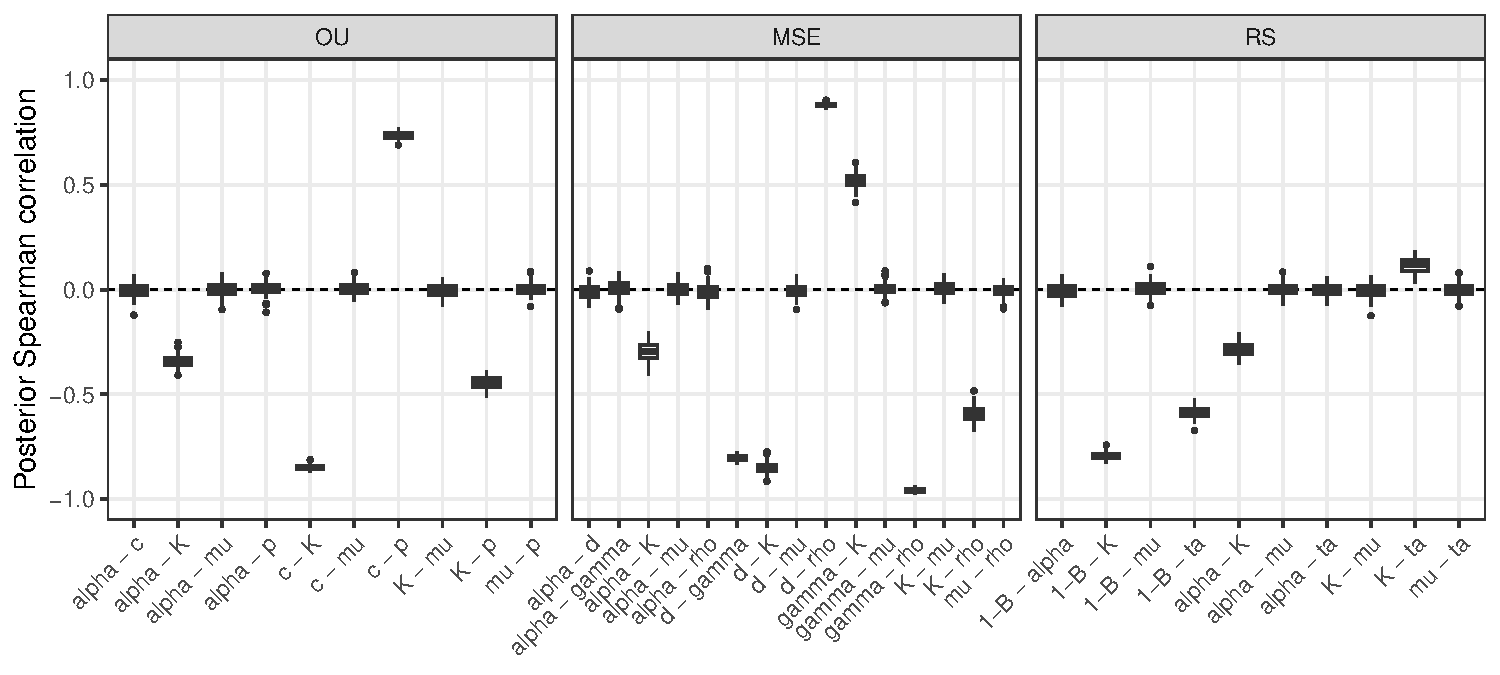
\includegraphics[width=0.9\linewidth]{images/posterior_parameter_correlations.pdf}
    \caption{Posterior dependence among ETAS parameters under correct specification. Boxplots show the distribution of within-catalogue posterior Spearman correlations across $100$ synthetic catalogues for each temporal form. Correlations are calculated from $1{,}000$ joint posterior samples per fitted catalogue. OU denotes Omori--Utsu, MSE modified stretched exponential, and RS rate-state.}
    \label{fig:simulation-posterior-correlation}
\end{figure}

\subsubsection{Posterior functional similarity under misspecification}\label{app:posterior-functional-tv}

\begin{figure} [H]
    \centering
    
\includegraphics[width=0.5\linewidth]{images/posterior_functional_tv.pdf}
    \caption{Posterior TV distance from the generating function across synthetic catalogues. Points show posterior medians, with bars indicating $95 \%$ credible intervals across $1{,}000$ joint posterior draws.}
    \label{fig:posterior-functional-tv}
\end{figure}

%=========================================================


\end{document}
